% ============================================================================
% 6 ARCHITECTURE AND SOLUTION DESIGN
% ============================================================================
\section{Architecture and Solution Design}
\label{sec:architecture}

Two artifacts implement workflow~(c) of \Cref{fig:workflows}: an evaluation
framework for data with reference labels and an annotation product for creating
reviewed labels where none exist.

\subsection{Evaluation framework}

The Python repository is separated by task. Configuration and prompt files
describe a run; method classes expose a common prediction interface; runners
handle API calls, retries and validation; evaluators read stored predictions and
write aggregate, per-example, per-label and error artifacts. The SciREX adapter
adds deterministic detokenization, document-window construction and offset
assertions. A production batch runner adds atomic sentence checkpoints,
configuration hashes, bounded parallelism, rate and call ceilings, token
accounting and idempotent resume. This separation is important: inference is
expensive and stateful, whereas scoring should be computationally inexpensive,
inspectable, and repeatable.

For ticket classification, an optional dense-retrieval component indexes
reviewed reference tickets with a pretrained sentence encoder and supplies the
nearest valid examples to the LLM prompt. The index manifest stores source and
artifact hashes, encoder identity, dimensions and column mappings. Reference
and evaluation data remain separate, and query-time exclusion by ticket ID and
normalized text provides an additional leakage safeguard. This component is a
retrieval baseline, not LLM fine-tuning, and remains excluded from reported
results until it is evaluated on an independent internal split.

\subsection{Human-in-the-loop annotation product}

The Streamlit application accepts pasted text, TXT, PDF, or an interactively
mapped CSV row. A user selects or copies a YAML use-case template, edits labels
and the complete schema-derived prompt, chooses an OpenAI-compatible or local
Ollama model, and runs pre-annotation. Suggestions are highlighted in context
and listed with exact character offsets, provenance, status and confidence
(\Cref{fig:tool}). Reviewers can confirm, relabel, delete, adjust or add spans.
The export retains immutable model predictions alongside final
\code{gold\_entities}, prompt hashes, token usage and the full review history.

\begin{figure*}[!t]
\centering
{\setlength{\fboxsep}{0pt}\setlength{\fboxrule}{0.4pt}%
 \fcolorbox{TUMLightGray}{white}{%
 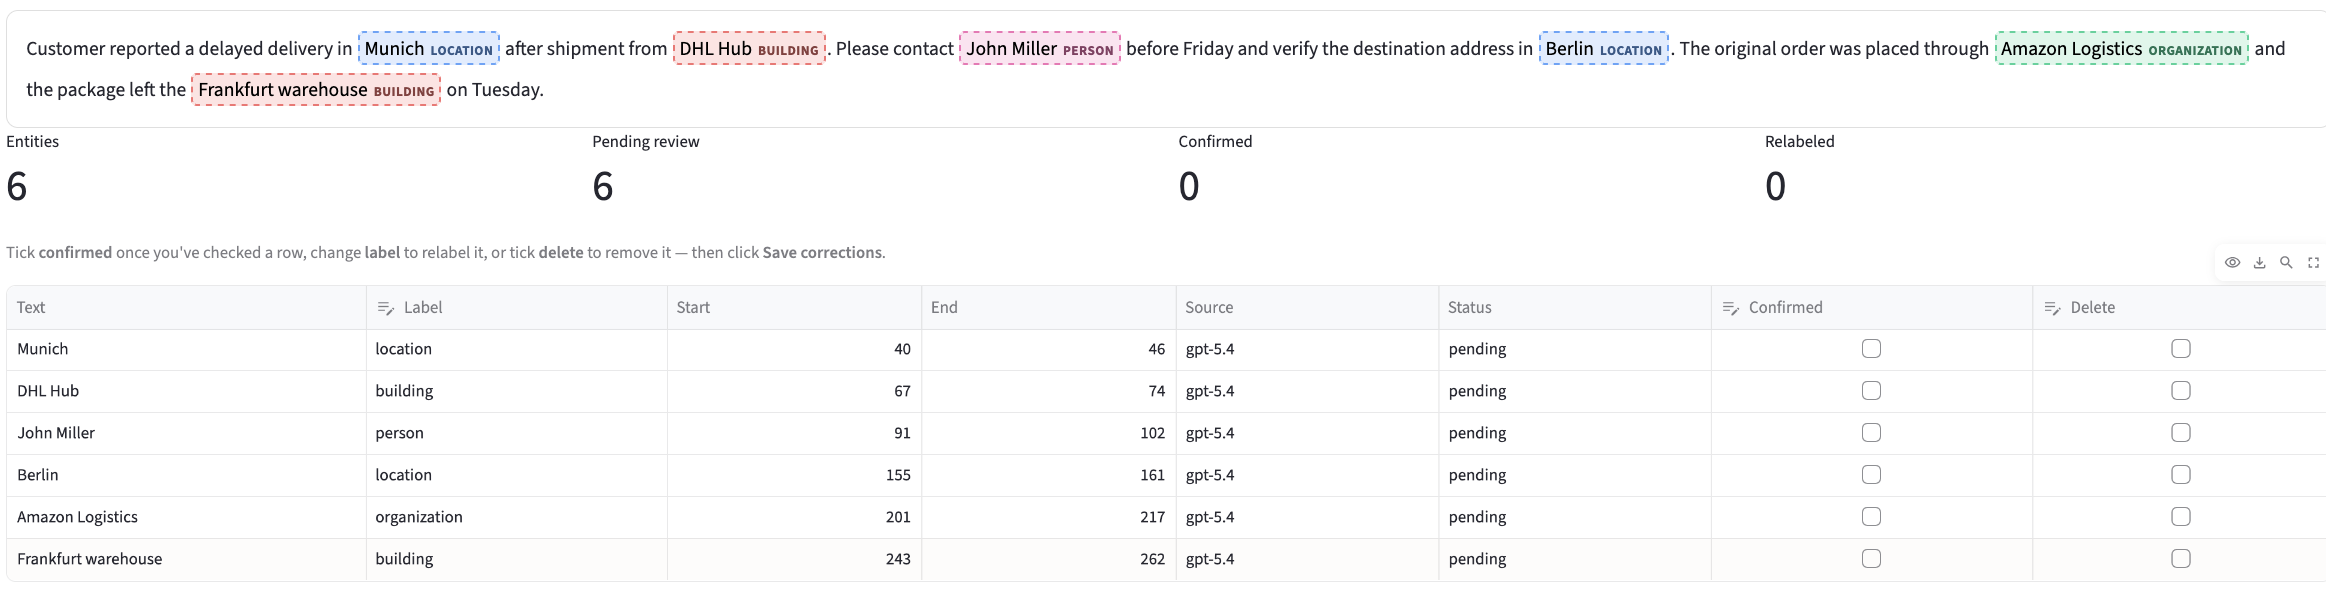
\includegraphics[width=\dimexpr\textwidth-0.8pt\relax]{figures/annotation_review.png}}}
\caption{Human review in the annotation product. Model spans are highlighted
in the source text and exposed as editable records; corrections and deletions
remain part of the audit trail rather than being overwritten.}
\label{fig:tool}
\end{figure*}

\paragraph{Reusable domain configuration.}
YAML templates currently cover general named entities, scientific IE and
internal support tickets. Each defines labels, descriptions, domain guidance
and optional routing destinations. The prompt suggestion is deterministic, so
it is reproducible and free, but the user can adapt it before inference. Custom
labels receive a generic starting definition instead of disabling the tool.

\paragraph{Optional classification before extraction.}
For tickets, the user selects either an LLM classifier or a local embedding
classifier. The LLM route uses a fully editable prompt, selects one department
from the allowed list and quotes ticket evidence. The local route maps a
reviewed CSV into ticket, department and ID columns, builds a pretrained
sentence-embedding index, retrieves the nearest reviewed tickets and applies a
similarity-weighted vote. It makes no routing LLM call, although extraction can
still use an LLM. The export records the classifier, prediction, confidence,
review decision and, for local routing, the encoder, source hash and neighbor
provenance. The reviewer confirms or corrects routing independently of entity
review. The evaluation page can summarize reviewer acceptance by classifier,
but this workflow measure is not independent classification accuracy; accuracy
requires labels assigned without seeing the prediction.

\paragraph{Long text and provenance.}
The tool processes sentences sequentially and converts their local spans to
document-level offsets. The user may choose a sentence limit for a quick test or
process the complete document. Sentence-local calls reduce context size and
make failure recovery precise, but they cannot resolve entities requiring
cross-sentence context. The batch runner addresses scale through checkpoints
rather than silently truncating documents.

\paragraph{Distribution and security boundary.}
A pinned Python 3.11 image, Dockerfile and Compose file make the product
independent of a particular IDE; a Dev Container remains optional. Credentials
enter at runtime through ignored environment or Streamlit-secret files and are
excluded from the Docker build context. Reviewed exports are mounted to the host.
This package is reproducible for evaluation, but it is not yet a multi-user
production service: authentication, role-based access, central persistence,
queues and tenant isolation remain outside the current implementation.
